\section{Arquitetura de sistema}
Na Figura~\ref{fig:46} é possível visualizar a arquitetura do sistema que indica os principais 
componentes deste software. Entre estes componentes é possível visualizar a aplicação frontend, 
onde esta realiza pedidos a uma aplicação backend e espera respostas. A aplicação backend é composta 
de uma api rest que receberá os pedidos e responderá aos mesmos, este backend é composto também por 
uma base de dados a qual vai receber queries e devolver dados para a aplicação api rest.

\begin{figure}[htb]
    \centering
    
    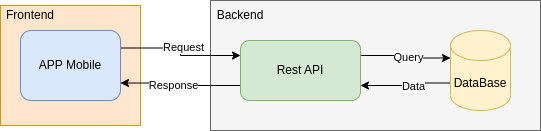
\includegraphics[width=\textwidth]{images/Arquiteturas/arquitetura_de_solucao.png}
    \caption{Arquitetura do sistema}
    \label{fig:46}
\end{figure}

\newpage

\subsection{Arquitetura de funcional}

Para especificar a implementação da api rest foi então criada uma arquitetura de 
backend(Figura~\ref{fig:47}), nesta arquitetura é possível visualizar que sempre que a api 
recebe um request este é redirecionado primeiramente para o router, o router tem como função 
identificar a rota a ser pedida e redirecionar para os respetivos middlewares. 

Os middlewares tem como função realizar todo o código necessário antes de proceder à execução 
do código de rota, os middlewares existentes são o SessionTokenValidator, este middleware tem 
como função validar a sessão do utilizador a realizar o pedido, de forma similar o middleware 
RefreshTokenValidator, valida a sessão principal do utilizador, por fim o middleware RoleValidator, 
tem como função validar se o utilizador que realiza o pedido tem cargos suficientes . 
Caso o pedido não seja impedido por nenhum middleware este é então direcionado para o 
controller.

O controller tem como função principal extrair os dados do pedido, validar os dados, verificando 
se os dados obrigatórios existem e encaminhar o pedido para o serviço, procedendo depois à formação 
da resposta e devolução da mesma. No serviço serão primeiramente aplicadas as regras de negócio para 
validar o conteúdo do pedido, caso o pedido não seja impedido por nenhuma das validações de 
regras de negócio, este então, em caso de necessidade, irá proceder à interação com base de dados, 
podendo esta realizar diversas interações como, obter dados, atualizar dados, apagar dados e inserir 
dados. Por fim a resposta é formada e devolvida como resposta ao pedido recebido.

\begin{figure}[htb]
    \centering
    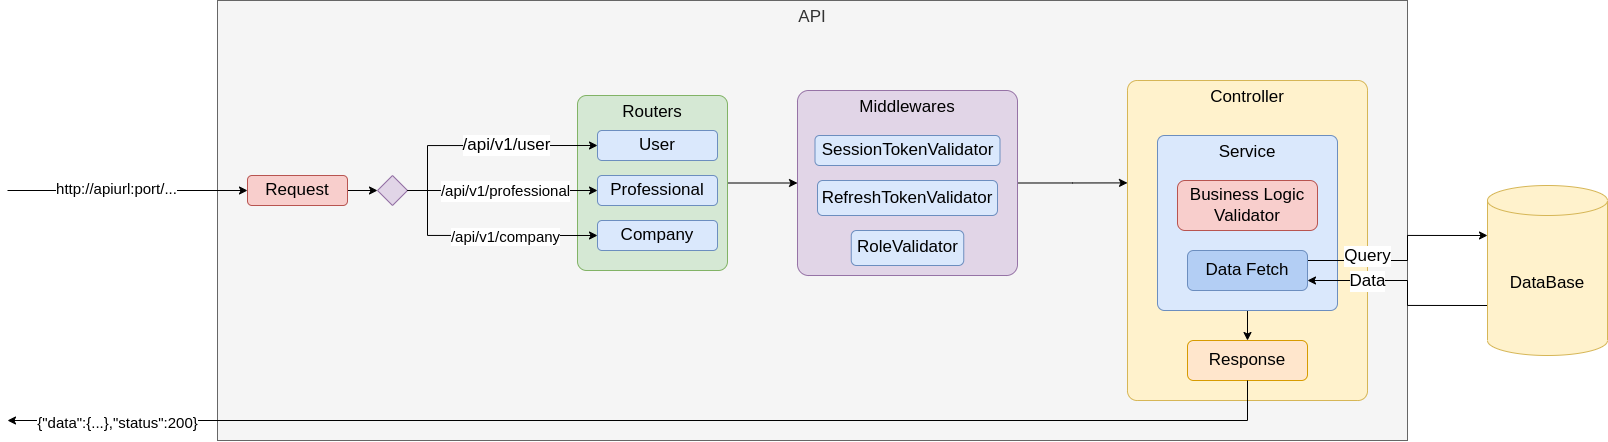
\includegraphics[width=\textwidth]{images/Arquiteturas/arquitetura_funcional.png}
    \caption{Arquitetura do funcional}
    \label{fig:47}
\end{figure}

\newpage

\subsection{Arquitetura de componentes}
Após a perceção de todas as necessidades da aplicação do frontend, foi então desenvolvida a 
arquitetura de componentes na qual estão contidos todos os serviços que deverão ser implementados na 
api frontend, identificando também qual ator poderá realizar estes pedidos.

\begin{figure}[htb]
    \centering
    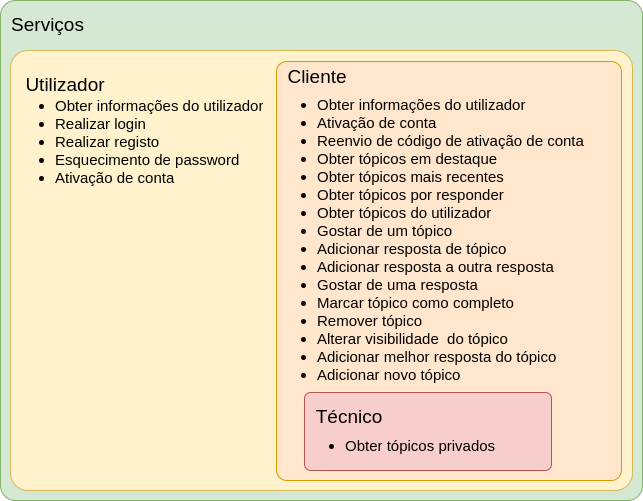
\includegraphics[width=0.7\textwidth]{images/Arquiteturas/arquitetura_de_componentes_final.png}
    \caption{Arquitetura de componentes}
    \label{fig:48}
\end{figure}

\newpage

\subsection{Tabela de endpoints}
De forma a evitar colisões de endpoints durante a implementação dos mesmos, foi então desenvolvida a 
tabela de endpoints que contém uma estrutura semelhante à arquitetura de componentes, mas que contém 
para cada serviço a rota e o método a utilizar.

% \usepackage{color}
% \usepackage{tabularray}
\definecolor{Concrete}{rgb}{0.952,0.952,0.952}
\begin{longtblr}
[
caption={Tabela de endpoints},
label={tab:19},
]{
  row{1} = {Concrete,c},
  hlines,
  vlines,
}
Serviço                                    & Ator       & Rota                                                             & Método \\
{Obter informações \\do utilizador}        & Cliente    & baseurl/client/:uid                                              & GET    \\
Realizar login                             & Utilizador & baseurl/login                                                    & POST   \\
Realizar registo                           & Utilizador & baseurl/register                                                 & POST   \\
{Esquecimento de \\password}               & Utilizador & baseurl/forgot-password                                          & GET    \\
Ativação de conta                          & Cliente & baseurl/client/:uid/activate                                     & POST   \\
{Reenvio de código \\de ativação de conta} & Cliente & baseurl/client/:uid/new-code                                     & GET    \\
{Obter tópicos em \\destaque}              & Cliente    & baseurl/client/topics/featured                                   & GET    \\
{Obter tópicos mais \\recentes}            & Cliente    & baseurl/client/topics/latest                                     & GET    \\
{Obter tópicos por \\responder}            & Cliente    & baseurl/client/topics/to-answer                                  & GET    \\
{Obter tópicos do \\utilizador}            & Cliente    & baseurl/client/topics                                            & GET    \\
{Obter tópicos \\privados}                 & Técnico    & baseurl/professional/topics/private                              & GET    \\
{Gostar de um \\tópico}                    & Cliente    & baseurl/client/topics/:topicId/like                              & PUT    \\
{Adicionar resposta \\a tópico}            & Cliente    & baseurl/client/topics/:topicId/answer                            & POST   \\
{Adicionar resposta \\a outra resposta}    & Cliente    & baseurl/client/answers/:answerId/                                & POST   \\
{Gostar de uma \\resposta}                  & Cliente    & baseurl/client/answers/:answerId/like                            & PUT    \\
{Marcar tópico \\como completo}            & Cliente    & baseurl/client/topics/:topicId/completed                         & PUT    \\
Remover Tópico                             & Cliente    & baseurl/client/topics/:topicId/                                  & DELETE \\
{Alterar visibilidade \\do tópico}         & Cliente    & baseurl/client/topics/:topicId/visibility                        & PUT    \\
{Adicionar melhor \\resposta do tópico}    & Cliente    & {baseurl/client/topics/:topicId/answers/\\:answerId/best-answer} & PUT    \\
Adicionar novo tópico                      & Cliente    & baseurl/client/topics/                                           & POST   
\end{longtblr}

\newpage
